\documentclass[12pt]{report}
\usepackage[a4paper,left=25mm, right=25mm, top=30mm, bottom=30mm]{geometry}
\usepackage[english]{babel}
\usepackage[utf8x]{inputenc}
\usepackage{amsmath}
\usepackage{graphicx}
\usepackage{wrapfig}
\usepackage{microtype}
\usepackage{setspace}
\usepackage{enumitem}
\usepackage{booktabs}

\usepackage[nottoc]{tocbibind}
\usepackage{natbib}
\usepackage[section]{placeins}

\usepackage{graphicx}
\usepackage{lscape}
\usepackage{amssymb}
\usepackage{epstopdf}
\usepackage{algorithm}
\usepackage{algorithmic}
\usepackage{subfig}
\usepackage{float}
\usepackage{wrapfig}
\usepackage{fancyhdr}
\usepackage{natbib}
\captionsetup{margin=10pt,font=small,labelfont=bf}
\usepackage[raggedright]{titlesec}
\usepackage{amsmath}
\usepackage{titlesec}
\usepackage{lipsum}
\usepackage{parskip} 
\usepackage{pdflscape}
\usepackage{rotating}
\usepackage{blindtext}
\usepackage{tabularx}
\usepackage{afterpage}
\usepackage{caption}
\usepackage{subfig}
\usepackage{graphicx}
\usepackage{epstopdf}
\usepackage[normalem]{ulem}
\useunder{\uline}{\ul}{}
\usepackage{longtable}

\setcounter{tocdepth}{5}
\setcounter{secnumdepth}{5}

% \renewcommand{\familydefault}{\sfdefault}
\usepackage[T1]{fontenc}
\usepackage{lmodern}

\setstretch{1.25}
\graphicspath{ {./images/} }
\bibliographystyle{apa} %agsm

\titleformat{\chapter}[display]
  {\normalfont\bfseries}{}{0pt}{\huge}
\begin{document}
\begin{titlepage}

   

    \title{ 
\includegraphics[scale=1.7]{utslogo.jpg}\\[1cm]  
    Faculty of Engineering and Information Technology\\[1.0cm] 
    \Large{\textbf{Human Body 3D Scanner (Virtual me)}}\\[1.0cm] 
    {Esteban Gabriel Andrade Zambrano\\
    Student Number: 12824583\\
    Project Number: AUT-21-04017\\
    Major: Mechanical and Mechatronics Engineering\\
    Supervisor: Dr. Teresa Vidal Calleja\\[2.0cm]
    \small{A 12 Credit Point Project submitted in partial fulfilment of the requirement for the Degree of Bachelor of Engineering}
    }
    \date{\today}   
   }
   
\end{titlepage}
\maketitle  
\cleardoublepage

%\addtocontents{toc}{\protect\thispagestyle{empty}}
\pagenumbering{roman}
\addtocontents{toc}{\protect}
\chapter*{Statement of Originality}
I, Esteban Gabriel Andrade Zambrano  declare that I am the sole author of this report, that I have not used fragments of text from other sources without proper acknowledgment, that theories, results and designs of others that I have incorporated into my report have been appropriately referenced and all sources of assistance have been acknowledged.\\[2 cm]
Refer to Appendix for signed statement of originality

\chapter*{Abstract}
\textbf{Human Body 3D Scanner (Virtual me) (12cp)}\\
Esteban Gabriel Andrade Zambrano - AUT-21-04017\\
Supervisor: Dr. Teresa Vidal Calleja\\
Major: Mechanical and Mechatronics Engineering.\\
\textbf{Objective}: Process recorded sensor data from a human body and create a scaled model of the scanned subject that can be used for clothing fitting.\\
\rule{\textwidth}{0.1pt}
The capability of scanning different models is critical for manu industries ranging from fashion to medical and manufacturing. Nevertheless many of the current implementations are extremely expensive. Hence it imposses a barrier for the technology.
Similarly, many of the current applications do not create extremely accurate models and in various occasions thgse models would be discarded.\\
Therefore, this project will create both hardware and software implementation for a human 3D scanner with a moderate budget as well as accurate results  in order to be able to produce accurate and scaled models of the scanned subject.
The proposed method for data acquisition will be with a custom rig. The rig will be a set of poles with cameras that will capture images from the person that is inside the rig. 
Additionally, a Lidar will be used to capture a PointCloud as well as an Image mof the subject inside the rig.\\
With the acquired images from all the cameras as well as the Lidar, a photogrammetry process will be used in order to obtain an initial mesh. This mesh is the result of the photogrametry reconstruction process.
Moreover, the initial mesh will be processes with a series of developed algorithms in a pipeline sequence. The pipeline will process the mesh with operations such as plane removal, outliers removal and clustering.\\
The Scaling will use the PointCloud from the Lidar as a reference and adjust the Scale and Pose of the processed mesh. Once the Mesh has been scaled appropiately with the reference PointCloud, a Poisson algorithm will be used in order to reconstruct and obtain the final scanned model.\\
The results in this report illustrate the process on how with a constrained data set, it is possible to obtain accurate scaled scanned model that can be used in many applications.
\enlargethispage{\baselineskip}
\chapter*{Acknowledgements}
I would like to acknowledge and thank my supervisor Dr. Teresa Vidal Calleja for her help and support throughout this project. I would also like to acknowledge and thank Dr. Cedric Le Gentil for all his guidance, support and input throughout the project development.
Furthermore, I would like to acknowledge Mr Asher Katz for his contributions in the development of the rig  and the image acquisition process component of the project.\\
On the other hand, I would also like to acknowledge Dr. Mark Liu as well as the UTS Robotics Institute for assitance and resources provided for the completion of this project.

Similarly, I would like to acknowledge the Open Source Community, as assets developed by this community helped in the development and completion of this project.

Finally, I would like to thank my family for their massive and ongoing support throughout this project and my studies. In equally importance I would like to thank God, who with his countless blessings have gave me the opportunity to develop and complete this project.
\tableofcontents
\listoffigures
\listoftables

%\thispagestyle{empty}
\newpage
\setcounter{page}{1}

\pagenumbering{arabic}
\chapter{Introduction}

\section{Reseach Question}
\textit{\large{"Human Body 3D Scanner: The development of software for 3D data reconstruction of a Human body scanner with multiple sensors" }}

\section{Project Contextualization}
The project is based on creating a Human Body 3D scanner.
It will have two specific streams that include the development of the mechatronic design of a 3D scanner for a human and the software development for 3D data reconstruction. 
This proposal is based on developing the software for 3D data modelling and reconstruction of the Scanned data.

Similarly, with the 3D reconstructed model of the human has the aim to be utilised to test different fashion clothing items. This has the intent to adjust the sizing of the clothes fittings based on the Scanned data. The clothing models will adjust automatically depending on the dimensions of the data of the scanned model. 
The project will have different stages that range from testing different sensors for data acquisition, testing different data stitching frameworks to the deployment of the software in the 3D scanner mechatronic device.

\section{Problem Definition}
Being able to scan different object and models is crucial for many industries. Many applications are in the used in the fashion industry, medical industry, manufacturing ,etc. However, many of the given implementations are extremely expensive , thus making the technology inaccessible for many companies and users in general. 
There are many forms of implementations, as there are multiple technologies in the market that facilitate the process in which several devices and software techniques are used. Nevertheless, there is no current industry application that maximises the potential use of the Human body 3D models.
Many of the challenges faced is that the software implementation for 3D reconstruction of the models is not particularly accurate, therefore creating imperfect models that on many occasions will need to be discarded.

Hence, this project component will contribute and develop the technology to produce software that will be able to produce accurate models from the gathered data from the sensors. These models will be utilised to try different fashion items and adapt the size fittings accordingly. 
With the competition of this project many stakeholders, industries and institutions could rely on accurate software that will  allow to create a 3D model of a person or object.


\enlargethispage{\baselineskip}

\section{Background}
The human society has the world comprehension of the surrounding world through visual perception. This principle allows differentiating distinctive kinds of shapes, objects, colours, textures, and the spatial pose of the surroundings.
Based on this information, it is possible to analyse the number of objects in a determined location, object type, object size, object pose in different coordinate frames. 
Thus, it impacts how as a society we interact with objects or scenes. As a result, it is essential to imitate this perception  to acquire real-world data in different formats that include:
\begin{itemize}[]
     \item RGB images
     \item Depth images
     \item 3D point clouds 
     \item Multispectral images
     \item Laser readings
\end{itemize}
All these acquire data can be obtained from a wide variety of commercial or industrial sensors. With this data, it will be possible to use computer processing techniques  to model the object or scene \citep*{murcia_monroy_mora_2018}.

\section{Applications}
In recent years, the use of 3D body scanners has gain importance in several industries. Within the fashion industry, it can aid clothes manufactures to obtain accurate body measurement data of body dimensions.
As mentioned by \citet*{sturm_bylow_kahl_cremers_2013}, this new technological approach has the potential to alternate the future of the fashion and clothing manufacturing industry.

With the rise of innovation of 3D image reconstruction, the interest  to gather precise measurements of humans has raised. Due to the fact, that in the clothing industry
is extremely important to create better fittings for different shapes of human bodies. 
Furthermore, virtual try-on solutions have gain popularity in physical and online retail stores \Citep*{spahiu_shehi_piperi_2014}.

On the other side, 3D scanners have gained participation in the medical industry. These systems are described as "non-invasive and low cost", thus making it appealing for epidemiological surveys and clinical uses. \Citep*{treleaven_wells_2007}
The geometrical measurements could be associated with shape, size, volume, and surface area of the body parts. It could aid to be a sustainable approach to screen children and patients with obesity, deformities, or specific anatomic defects. 
Therefore, it will ease the diagnose process and allow to treat and monitor medical conditions holistically and improve the life quality of patients with non-invasive tests.
The table below illustrates the use of a 3D scanner in the medical field with the purpose to identify and monitor various medical conditions. 
From which the diagnose, treatment and monitor procedures will differ based on the acquired data.
\begin{table}[ht]
    \centering
    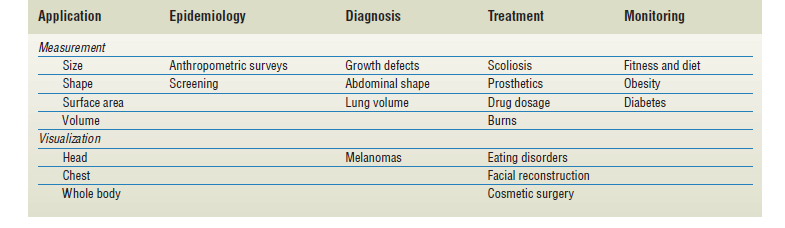
\includegraphics[width=15cm]{table1.png}
    \caption{3D Scanning Applications}\cite[]{treleaven_wells_2007}.
\end{table}

\section{Overview}
As mentioned before, project consists of developing a 3D scanner that is allowed to scan person and be able to use that data in order to be able to virtually fit different clothing.
This capstone project mainly focuses on the software and processing of the data for the 3D reconstruction.

The aim of this project is to develop algorithms and an implementation pipeline that will use the acquired image data as well as the reference pointcloud data in order to produce an accurate
and appropiately scaled 3D reconstructed model of a person.\\
This is reconstructed ans scaled model of the scanned person, is intended to be utilised as the model for testing virtual clothe fitting and be able to correctly determine the size of the garments. 
This technology could have a massive industry in the clothing industry and online retailers as this could solve an issue with the returns policy due to incorrect sizing for different customers groups.
\subsection{Methodology}
To achive the aim, a rig will be used to capture the data. The Rig will consist of a set of poles with multiple cameras. Furthermore a Lidar Intel RealSense L515 will be used to capture another image an the corresponding pointcloud that will be used for reference.
Once the rig captures the data (28 images) as well as the lidar data(1 image, 1 pointcloud), the images will be processed with photogrammetry approach with Meshroom. 
The Processed data from Meshroom will produce a preprocessed reconstruction mesh. 

After this the mesh will be processed in the developed algorithmic pipeline and it will be properly scaled with the reference pointcloud from the Lidar. 
Once the mesh has been processed and scaled, it will be reconstructed appropiatelyand it will generate a final model of the scanned person with the with only the necessary components and appropriate scale.

Once the process is completed the mesh will be saved to disk as a ply file that can be later use in other applications such as clothing fitting. 

\subsection{Structure}
This Report will start with a literature review in order to analyse and fully understand the algorithms and techniques that are used in both components. 
It will help to understand the techniques used in the photogrammetry step and the developed algorithm pipeline.

Following this, details will be presented and illustrated as to how the process is carried out and the results that were obtained from different data sets.
It will fully ilustrated how to import the data to Meshroom, what parameters are required to add and modify in order to change the most robust reconstruction. There will be an indetail explanation of what each step executes.

Furthermore, there will be an detailed explanation of the algorithm pipeline for data processing. Here it will be explain what each component is expected to execute as well as how it was created and wrapped into a framework.

\chapter{Literature Review}
Being able to scan different objects and subjects has been a challenging task for researchers. Getting an accurate spatial location of the objects is crucial for this type of application.
The use of 3D point clouds has facilitated this process as it allowed to obtain the following parameters:
\begin{itemize}[]
  \itemsep0em 
  \item Depth
  \item Intensity
  \item Pulse width
  \item Light echo
\end{itemize}
This information can be obtained with different kind of sensors. There is a wide variety of off the shelf sensors that can provide 3D point clouds. 
These sensors could either be stereo or multiview vision cameras, lasers, time-of-flight sensors (\textit{TOF}) and structured light sensors as stated by \Citet*{murcia_monroy_mora_2018}.

Many Scanning devices will use single or multiple of the above-mentioned sensors to acquire data. Once the data is obtained, it essential to have a framework for 3D data modelling and reconstruction.
The principle behind 3D data reconstruction is obtained with data fusion from RGB-D sensors. This kind of sensors provide 3 channels images RGB (red, green, blue) and the depth images are mapped to each pixel. Based on this data, 3D point clouds could be generated for data reconstruction.

Similarly many other scanning devices use photogrammetry as a technique in order to do the reconstruction. In this particular project Meshroom was used as a 3D photogrammetry reconstruction software.

Moreover, several open source libraries were used in order to process and scale the draft mesh. These open source libraries include PCL and Open3D. From these several algorithms were used that aid in the data processing and these will be explained below. 
\enlargethispage{\baselineskip}

\section{Photogrammetry}
Photogrammetry is decribed as the associated techniques with performing measurements of real-world objects and terrain features from images as mentioned by \Citet*{photogrammetry_def}.
Many of the applications include the quantification of distances, volumes,areas, heights, 3D topographic mapping, measuring of objects, extracion of 3D pointcloud for surfaces reconstruction as well as the generation of orthophotographs and digital elevation models.\Citep*{photogrammetry_def}.

In recent years, with the development of technologies pairing computer vision concepts \& algorithms and photogrammetry specifically \textit{Structure from Motion-Multiview Stereo (\textbf{SfM-MVS})}
has led to significant advances in 3D surface Reconstruction from images \Citep*{photogrammetry_def}.

The key principle behind all the photogrammetric measurements is associated with the mathematical \& geometrical reconstruction of the path of light rays from the object to the sensor camera in the exact moment of data image acquisition.
Thus, the fundamental concept of photogrammetry is the undertanding of geometric characteristics of a single photograph.

\begin{figure}[h]
  \centering
  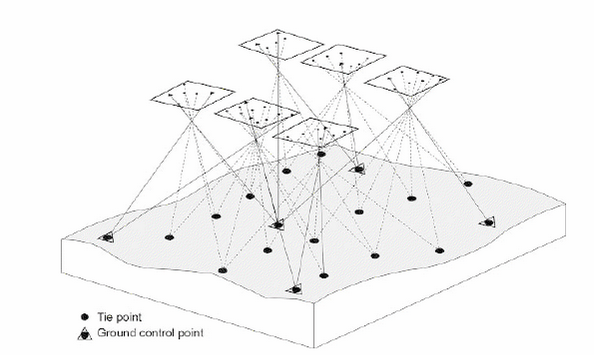
\includegraphics[width=0.8\textwidth]{photogrammetry.png}
  \caption{Photogrammetry Principle Illustration}\cite[]{photogrammetry_def}
  \label{fig:photogrammetry_principle} 
\end{figure}

\section{Meshroom}
Meshroom is a free, open-source 3D Reconstruction Software based on the AliceVision framework \Citep*{meshroom}.
AliceVision is a software framework based on photogrametric computer vision.  which focuses on the development of 3D Reconstruction and Camera Tracking Algorithms.
It aims to provide robust software foundation with novel computer vision algorithms that can be analysed, tested and reused.\\
Meshwoom was developed as collobaration project between industry and academia in order to develop cutting-edge algorithms that are robust and of high quality which are crucial for production environments.

\subsection{Components Pipeline}
Meshroom can be downloaded and used in both Windows and Linux and it will require a powerfull CPU in order to have adequate performance. Also it will require an Nvidia GPU as it requires to run CUDA for different nodes and components.
Once meshroom is downloaded it can run in either platform. When it is executed the Meshroom GUI will appear and it will be similar to figure \ref{fig:meshroom_gui}

\begin{figure}[h]
  \centering
  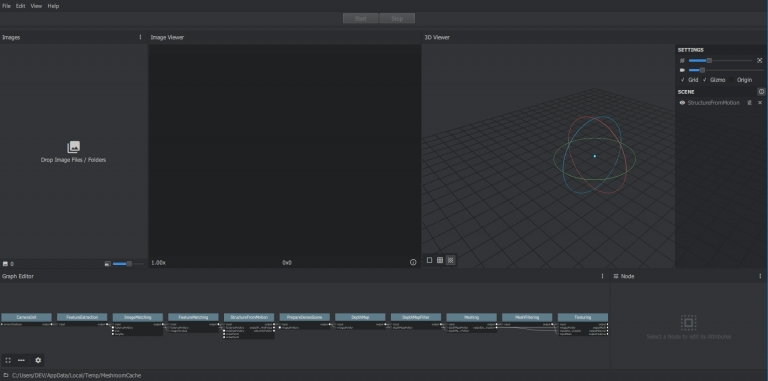
\includegraphics[width=1\textwidth]{meshroom_gui.jpg}
  \caption{Meshroom Graphical User Interface}\cite[]{meshroom}
  \label{fig:meshroom_gui} 
\end{figure}

\newpage
As mentioned before, meshroom is based on AliceVision's Framework. Therfore it follows a photogrametric pipeline for 3D reconstruction. 
This pipeline will have the following components:
\begin{itemize}
  \item Natural Feature Extraction
  \item Image Matching
  \item Features Matching
  \item Structure from Motion
  \item Depth maps estimation
  \item Meshing
  \item Texturing
  \item Localization
\end{itemize}

The pipeline will be included into Meshroom GUI and it will be used in the nodes. All the components in Meshroom will be embedded into different individual nodes that will be executed and produce individual results that will be send to the next node along in the pipeline.
As the nodes represent specific components of the reconstruction pipeline, these should be executed in a defined order.\\
The nodes in the defined order to reconstruct a 3D model from images include:
\begin{enumerate}
  \item Camera Initialization 
  \item Feature Extraction
  \item Image Matching
  \item Feature Matching
  \item Structure From Motion
  \item Prepare Dense Scene
  \item Depth Map
  \item Depth Map Filter
  \item Meshing
  \item Mesh Filtering
  \item Texturing
\end{enumerate}

\subsubsection{Camera Initialization}
Camera Initialization or \textit{"CameraInit"} loads the image metadata, sensor information, camera parameters and it will  generate viewpoints based on the images.
It is possible to use a mixture of cameras \& focal lengths. This node will generate a groups of intrinsics that are based on the images metadata, these grooup os intrinsics can be adjusted if the cameras have been fully calibrated.
The intrinsic include the camera matrix  which includes the focal length ($f_x$,$f_y$) and principal point ($x_0$,$y_0$).
\begin{equation*}
  Camera Intrinsics = 
  \begin{pmatrix}
  f_x & 0 & x_0 \\
  0 & f_y & y_0 \\
  0 & 0 & 1
  \end{pmatrix}
\end{equation*}
\label{equ:camera_intrisics}

% Please add the following required packages to your document preamble:
% \usepackage{graphicx}
\begin{table}[h!]
  \centering
  \resizebox{\textwidth}{!}{%
  \begin{tabular}{|l|l|}
  \hline
  Viewpoints Input &
    \begin{tabular}[c]{@{}l@{}}viewpoints (1 Element for each loaded image) \\ - ID \\ - Pose ID \\ -  Image Path \\ - Intrinsic: Internal Camera Parameters (Intrinsic ID) \\ - Rig  (-1 - 200) \\ - Rig Sub-Pose: Rig Sub-Pose Parameters (-1 - 200)\\  - Image  Metadata: (list of metadata elements)\end{tabular} \\ \hline
  Intrinsic Camera Intrinsics &
    \begin{tabular}[c]{@{}l@{}}(1 Element for each loaded image) - ID - Initial Focal Length:  Initial Guess on the Focal Length \\ - Focal Length: Known/Calibrated Focal  Length \\ - Camera Type: pinhole’, ‘radial1’, ‘radial3’, ‘brown’,  ‘fisheye4’ \\ - \#Make: Camera Make (not included in this build, commented  out) \\ - \#Model: Camera Model \\ - \#Sensor Width: Camera Sensor Width \\ -  Width: Image - Width (0-10000) \\ - Height: Image Height (0-10000) - Serial  Number: Device Serial Number (camera and lens combined) \\ - Principal  Point: X (0-10000) Y(0-10000)\\ - DistortionParams: Distortion Parameters \\ -  Locked(True/False): If the camera has been calibrated, the internal  camera parameters (intrinsics) can be locked. It should improve  robustness and speedup the reconstruction.\end{tabular} \\ \hline
  Sensor Database &
    Camera sensor width database path \\ \hline
  Default Field Of View &
    Empirical value for the field of view in degree 45° (0°-180°) \\ \hline
  Verbose Level &
    verbosity level (fatal, error, warning, info, debug, trace) \\ \hline
  Output SfMData File &
    …/cameraInit.sfm \\ \hline
  \end{tabular}%
  }
  \caption{Meshroom CameraInit Node }
  \label{tab:CameraInit}
  \end{table}

\subsection{Feature Extraction}
% https://meshroom-manual.readthedocs.io/en/latest/feature-documentation/core/pipelines/photogrammetry.html
The key objective of this node is to extract distinctive pixel groups, which are to a certain extend invariant to a change in camera viewpoints during the image acquisition process.
Thus, a feature in this scene should have similar features descriptors in all the captures images.

One of the most used feature detection method is \textbf{SIFT} \textit{(Scale-invariant feature transform)} algorithm. 
The objective of SIFT is to extract discriminative patches in an initial image that later can be compared to discriminative patches of a second image, irrespective of scale, rotation and translation \Citep*{Lowe2004}.
As a relevant detail is only present at a specific scale, the extracted patches are centered around the point of interests. 
Therefore, the SIFT invarience can be used to deal with image transformations that occur when the viewpoints change during image acquisition.

Based on the representation of one image at different scales, SIFT is able to compute scale-space maxima of the Laplacian Representation. This is a defined image energy-based representation, using the differences of Gaussians.
This Maxima is associated to the points of interest in the image. 
Once this is processed, it samples for each of the this maxima a square image patch, whose origin is the maximum and "x" direction is the dominant gradient at the origin as suggested by \Citet*{Lowe2004} and\Citet*{Otero2014} .
For each keypoint, a description of these patches is associated. 

The description consists of statistics of gradients which is computed in regions around the keypoint. The size of the region is defined by the keypoint scale and the orientation by the dominant axis.
 It is also frequently stored in 128 bits.
 \enlargethispage{\baselineskip}

The number of extracted features could vary as a result of texture complexity, from one image to other ones or in different image sections. Hence, a post-filtering step controls the number of extrated features to a specified limit. 
Furthermore, grid filtering is used to ensure an even repartition in the image.


\begin{table}[h!]
  \centering
  \resizebox{\textwidth}{!}{%
  \begin{tabular}{|l|l|}
  \hline
  \multicolumn{1}{|c|}{Name} & Description                                                          \\ \hline
  Input                      & SfMData file.                                                        \\ \hline
  Describer Types &
    Describer types used to describe an image. ‘sift’, ‘sift*float’, ‘sift*upright’, ‘akaze’, ‘akaze*liop’, ‘akaze*mldb’, ‘cctag3’, ‘cctag4’, ‘sift*ocv’, ‘akaze*ocv’ \\ \hline
  Describer Preset &
    Control the ImageDescriber configuration (low, medium, normal, high, ultra). Configuration “ultra” can take long time ! \\ \hline
  Force CPU Extraction       & Use only CPU feature extraction.                                     \\ \hline
  Max Nb Threads &
    Specifies the maximum number of threads to run simultaneously (0 for automatic mode). (0-24) 0 \\ \hline
  Verbose Level              & verbosity level (fatal, error, warning, info, debug, trace).         \\ \hline
  Output Folder              & Output path for the features and descriptors files (*.feat, *.desc). \\ \hline
  \end{tabular}%
  }
  \caption{Meshroom FeatureExtraction Node Settings}
  \label{tab:FeatureExtraction}
  \end{table}

  
\subsection{Image Matching}
The principle behind this node is to find images that point to the same areas of interest. Therefore, image retrieval techniques are implemented with the purpose of finding images 
that share content without the demand of resolving all the  detailed feature matches. Hence, the goal is to simplify the image in a compact image descriptor. This allows to efficiencly compute the distance between all images descriptors.

A vocabulary tree is one of the widely used methodologies to generate the image descriptor. It works by passing all the extracted features descriptors into it. Then it performs a classification process, which compares their descriptors to the ones on each node of the vocabulary tree as mentioned by \Citet*{Nister2006}.
Each feature descriptor is associated with one leaf, which can be stored with an standard index (\textit{The index of this leaf in the tree}).Thus, the collection of leaves indices represents the image descriptor \Citep*{Nister2006}.

% Please add the following required packages to your document preamble:
% \usepackage{graphicx}
\begin{table}[h!]
  \centering
  \resizebox{\textwidth}{!}{%
  \begin{tabular}{|l|l|}
  \hline
  \multicolumn{1}{|c|}{\textbf{Name}} & \multicolumn{1}{c|}{\textbf{Description}}                               \\ \hline
  Image                               & SfMData file                                                            \\ \hline
  Features Folders                    & Folder(s) containing the extracted features and descriptors             \\ \hline
  Tree                                & Input name for the vocabulary tree file ALICEVISION\_VOCTREE            \\ \hline
  Weights &
    Input name for the weight file, if not provided the weights will be computed on the database built with the provided set \\ \hline
  Minimal Number of Images &
    \begin{tabular}[c]{@{}l@{}}Minimal number of images to use the vocabulary tree. \\ If we have  less features than this threshold, we will compute all matching  combinations\end{tabular} \\ \hline
  Max Descriptors                     & Limit the number of descriptors you load per image. Zero means no limit \\ \hline
  Nb Matches &
    The number of matches to retrieve for each image (If 0 it will retrieve all the matches) 50 (0-1000) \\ \hline
  Verbose Level                       & verbosity level (fatal, error, warning, info, debug, trace)             \\ \hline
  Output List File                    & Filepath to the output file with the list of selected image pairs       \\ \hline
  \end{tabular}%
  }
  \caption{Meshroom Image Matching Node}
  \label{tab:ImageMatching}
  \end{table}



\subsection{Feature Matching}
The key component of feature matching node is to be able to match all features between potential image pairs.
Initially, the node performs a photometric process that creates matches between the descriptors from 2 separe images. For each feature in image "A", a list of potential features in image "B" is generated.
The descriptor space is not linear and defined space, which causes uncertainty in the validity of the matches due to the absolute distance values. 
Furthermore, in order to remove bad candidates, an assumption process associates only one valid match in the other image.
Hence, for each feature descriptor on Image "A", two of the closests descriptors in the image are used with a relative threshold between them which provides a robust criteria as mentioned by \Citet*{Lowe2004}.

This process will provide a photometric list of feature matching candidates. Afterwards, the images features positions are used in a geometrica
filtering process that uses epipolar geometry in an outlier detection framework, which is RANSAC (\textit{"Random Sample Consensus"}).
Moreover, a random selection process uses a small set of feature correspondances and it computers either the fundamental or essential matrix. 
Once this process is completed, the number of features verifies and validates this model and iterates through the RANSAC framework \Citep*{FLANN2009}.

% Please add the following required packages to your document preamble:
% \usepackage{graphicx}
% \usepackage[normalem]{ulem}
% \useunder{\uline}{\ul}{}
\begin{table}[h!]
  \centering
  \resizebox{\textwidth}{!}{%
  \begin{tabular}{|l|l|}
  \hline
  \multicolumn{1}{|c|}{\textbf{Name}} &
    \multicolumn{1}{c|}{\textbf{Description}} \\ \hline
  Input &
    SfMData file \\ \hline
  Features Folder &
     \\ \hline
  Features Folders &
    Folder(s) containing the extracted features and descriptors \\ \hline
  Image Pairs List &
    Path to a file which contains the list of image pairs to match \\ \hline
  Describer Types &
    Describer types used to describe an image **sift**'/ 'sift\_float'/ 'sift\_upright'/ 'akaze'/ 'akaze\_liop'/ 'akaze\_mldb'/ 'cctag3'/ 'cctag4'/ 'sift\_ocv'/ 'akaze\_ocv \\ \hline
  Photometric Matching Method &
    \begin{tabular}[c]{@{}l@{}}For Scalar based regions descriptor \\ * BRUTE\_FORCE\_L2: L2  BruteForce matching\\ * ANN\_L2: L2 Approximate Nearest Neighbor  matching \\ * CASCADE\_HASHING\_L2: L2 Cascade Hashing matching\\ *  FAST\_CASCADE\_HASHING\_L2: L2 Cascade Hashing with precomputed hashed  regions (faster than CASCADE\_HASHING\_L2 but use more memory) \\ For Binary  based descriptor  \\ * BRUTE\_FORCE\_HAMMING: BruteForce Hamming matching\end{tabular} \\ \hline
  Geometric Estimator &
    Geometric estimator: (acransac:  A-Contrario Ransac //  loransac: LO-Ransac (only available for fundamental\_matrix model) \\ \hline
  Geometric Filter Type &
    Geometric validation method to filter features matches: **fundamental\_matrix** // essential\_matrix // homography\_matrix /// homography\_growing // no\_filtering' \\ \hline
  Distance Ratio &
    Distance ratio to discard non meaningful matches 0.8 (0.0 - 1) \\ \hline
  Max Iteration &
    Maximum number of iterations allowed in ransac step 2048 (1 - 20000) \\ \hline
  Max Matches &
    Maximum number of matches to keep (0 - 10000) \\ \hline
  Save Putative Matches &
    putative matches (True/False) \\ \hline
  Guided Matching &
    the found model to improve the pairwise correspondences (True/False) \\ \hline
  Export Debug Files &
    debug files (svg/ dot) (True/False) \\ \hline
  Verbose Level &
    verbosity level (fatal, error, warning, info, debug, trace) \\ \hline
  Output Folder &
    Path to a folder in which computed matches will be stored \\ \hline
  \end{tabular}%
  }
  \caption{Meshroom Feature Matching Node}
  \label{tab:FeatureMatching}
  \end{table}

\subsection{Structure From Motion}

% Please add the following required packages to your document preamble:
% \usepackage{graphicx}
% \usepackage[normalem]{ulem}
% \useunder{\uline}{\ul}{}
\begin{table}[]
  \centering
  \resizebox{\textwidth}{!}{%
  \begin{tabular}{|l|l|}
  \hline
  \textbf{Input}                      & \textbf{SfMData file}                                                                              \\ \hline
  Features Folder                     & Folder(s) containing the extracted features and descriptors.                                       \\ \hline
  Matches Folders                     & Folder(s) in which computed matches are stored.                                                    \\ \hline
  Describer Types &
    Describer types used to describe an image. ‘sift’, ‘sift*float’, ‘sift*upright’, ‘akaze’, ‘akaze*liop’, ‘akaze*mldb’, ‘cctag3’, ‘cctag4’, **’siftocv’, ‘akazeocv’ \\ \hline
  Localizer Estimator                 & Estimator type used to localize cameras (acransac, ransac, lsmeds, loransac, maxconsensus).        \\ \hline
  Observation Constraint &
    \begin{tabular}[c]{@{}l@{}}Observation constraint mode used in the optimization: \\ Basic:  Use standard reprojection error in pixel coordinates, \\ Scale: Use  reprojection error in pixel coordinates but relative to the feature  scale\end{tabular} \\ \hline
  Localizer Max Ransac Iterations     & Maximum number of iterations allowed in ransac step. (1-20000) 4096                                \\ \hline
  Localizer Max Ransac Error &
    \begin{tabular}[c]{@{}l@{}}Maximum error (in pixels) allowed for camera localization  (resectioning).\\ If set to 0, it will select a threshold according to the  localizer estimator used (if ACRansac, it will analyze the input data  to select the optimal value). (0.0-100-0) 0.0\end{tabular} \\ \hline
  Lock Scene Previously Reconstructed & This option is useful for SfM augmentation. Lock previously reconstructed poses and intrinsics.    \\ \hline
  Local Bundle Adjustment &
    It reduces the reconstruction time, especially for large datasets  (500+ images) by avoiding computation of the Bundle Adjustment on areas  that are not changing. \\ \hline
  LocalBA Graph Distance              & Graph-distance limit to define the Active region in the Local Bundle Adjustment strategy. (2-10) 1 \\ \hline
  Maximum Number of Matches &
    \begin{tabular}[c]{@{}l@{}}Maximum number of matches per image pair (and per feature type).\\  This can be useful to have a quick reconstruction overview. 0 means no  limit. (0-50000) 1\end{tabular} \\ \hline
  Minimum Number of Matches &
    \begin{tabular}[c]{@{}l@{}}Minimum number of matches per image pair (and per feature type). \\ This can be useful to have a meaningful reconstruction with accurate  keypoints. 0 means no limit. (0-50000) 1\end{tabular} \\ \hline
  Min Input Track Length              & Minimum track length in input of SfM (2-10)                                                        \\ \hline
  Min Observation For Triangulation &
    \begin{tabular}[c]{@{}l@{}}Minimum number of observations to triangulate a point. \\ Set it to 3  (or more) reduces drastically the noise in the point cloud, but the  number of final poses is a little bit reduced (from 1.5\% to 11\% on the  tested datasets). (2-10)\end{tabular} \\ \hline
  Min Angle For Triangulation         & Minimum angle for triangulation. (0.1-10) 3.0                                                      \\ \hline
  Min Angle For Landmark              & Minimum angle for landmark. (0.1-10) 2.0                                                           \\ \hline
  Max Reprojection Error              & Maximum reprojection error. (0.1-10) 4.0                                                           \\ \hline
  Min Angle Initial Pair              & Minimum angle for the initial pair. (0.1-10) 5.0                                                   \\ \hline
  Max Angle Initial Pair              & Maximum angle for the initial pair. (0.1-60) 40.0                                                  \\ \hline
  Use Only Matches From Input Folder &
    Use only matches from the input matchesFolder parameter. Matches folders previously added to the SfMData file will be ignored. \\ \hline
  Use Rig Constraint                  & Enable/Disable rig constraint.                                                                     \\ \hline
  Force Lock of All Intrinsic Camera Parameters. &
    \begin{tabular}[c]{@{}l@{}}Force to keep constant all the intrinsics parameters of the  cameras (focal length, principal point, distortion if any) during the  reconstruction. \\ This may be helpful if the input cameras are already  fully calibrated.\end{tabular} \\ \hline
  Filter Track Forks &
    \begin{tabular}[c]{@{}l@{}}Enable/Disable the track forks removal. \\ A track contains a fork  when incoherent matches lead to multiple features in the same image for a  single track.\end{tabular} \\ \hline
  Initial Pair A                      & Filename of the first image (without path).                                                        \\ \hline
  Initial Pair B                      & Filename of the second image (without path).                                                       \\ \hline
  Inter File Extension                & Extension of the intermediate file export. (‘.abc’, ‘.ply’)                                        \\ \hline
  Verbose Level                       & Verbosity level (fatal, error, warning, info, debug, trace).                                       \\ \hline
  Output SfMData File                 & Path to the output sfmdata file (sfm.abc)                                                          \\ \hline
  Output SfMData File                 & Path to the output sfmdata file with cameras (views and poses). (cameras.sfm)                      \\ \hline
  Output Folder                       & Folder for intermediate reconstruction files and additional reconstruction information files.      \\ \hline
  \end{tabular}%
  }
  \caption{Meshroom StructureFromMotion Node}
  \label{tab:StructureFromMotion}
  \end{table}



\subsection{Prepare Dense Scene}
% https://www.tablesgenerator.com/latex_tables#
\subsection{Depth Map}

% https://meshroom-manual.readthedocs.io/en/latest/feature-documentation/core/pipelines/photogrammetry.html

\subsection{Depth Map Filter}

\subsection{Meshing}

\subsection{Mesh Filtering}

\subsection{Texturing}

\subsection{Localization}
% https://alicevision.org/#photogrammetry/localization

\section{PCL}

\section{Open3D}

\section{Dynamic Fusion}
Dynamic fusion is based on three different technologies focused on 3D scanning and data reconstruction. These techniques are: 

\begin{description}[style=nextline]
  \item[DART (Dense Articulated Real-Time Tracking)] This technology is specialised on Real-Time body template skeleton tracking.
  \item[Animation Cartography] It is a 3D reconstruction technique focused on intrinsic data reconstruction of shapes and motions. 
  \item[Kinect Fusion] This technology is applied for real-time tracking and condensed surface mapping. It is intended to be used in static scenes and objects with only a moving camera sensor. 
\end{description} 

\vspace{5mm}

\begin{wrapfigure}{r}{0.475\textwidth} %this figure will be at the right
    \centering
    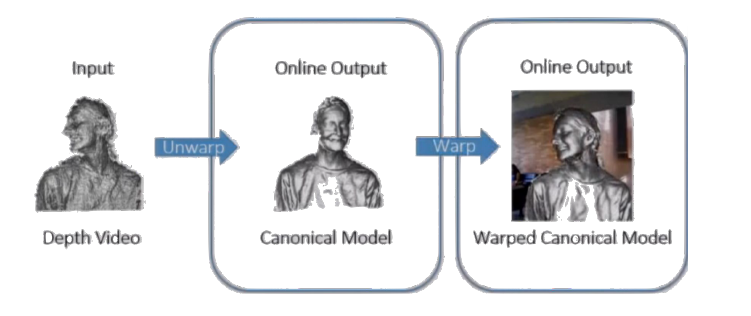
\includegraphics[width=0.475\textwidth]{IMG_0073.png}
    \caption{Transformation Between Depth Video to Warped canonical Model} \cite[]{newcombe_fox_seitz_2015}.
\end{wrapfigure}
The focal point of the 3D data reconstruction feature of \textit{Dynamic Fusion}  is that it will look for a solution for the volumetric flow based on the gathered data.
As mentioned by \Citet*{newcombe_fox_seitz_2015} there will be a transformation of the state of the scene at each time interval to a fixed canonical frame.
The created canonical frame is described as the initial frame that is obtained from the non-rigid object that has been detected and tracked. The shape of the detected object is defined as "canonical model" which is the corresponding shape of the object in the canonical frame. 
Therefore, the canonical model will be utilised as a reference model for all the subsequent frames. From this approach, there will be progressing adjustment on the canonical model and frames, as more data is acquired.
With the new refinements each point in the canonical frame, the point clouds will be transformed and updated to the new location in real-time based on the received data.

The data acquired from sensors that include RGB and Depth images will help to determine the warp parameters. Based on the determined warp parameters the volumetric flow field can be stipulated.
The state of the wrap field W\textsubscript{t} is defined as a function of time. It is modelled by the values of a set of \textit{"n"} deformation nodes, which are described as the points or pixels in the actual image.
The image below describes the process in which the canonical model and frame are determined based on the initial frame and depth data. 
\begin{figure}{}%this figure will be at the right
    \centering
    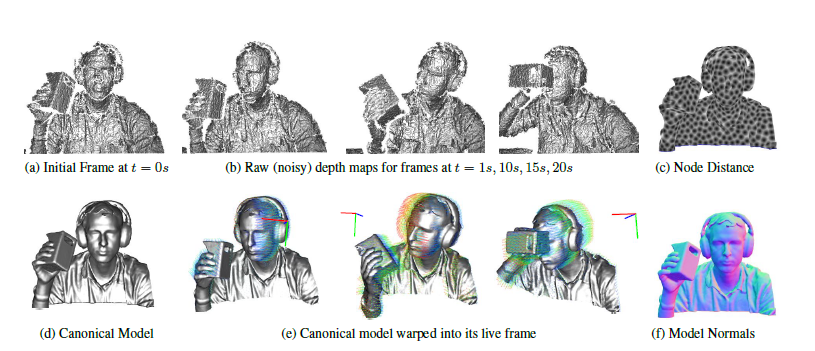
\includegraphics[width=0.7\textwidth]{dynamicfusion2.png}
   \caption{Dynamic Fusion methodology}\cite[]{newcombe_fox_seitz_2015} 
\end{figure}


The State of the warp field W\textsubscript{t} can be modelled with the below equation.
\[N_{warp}^t=\{dg_v,dg_w,dg_{se3}\}t\]
\begin{itemize}[label =]
  \item $dg_{v}$: is described as the 3D position of each node in the canonical frame. 
  \item $dg_{se3}$: is the Special Euclidian transformation where $T_{ic}=dg_{se3} ^ {i}$ is the rigid transformation for every node $i$.
  \item $dg_{w}$: It controls the extended impact of the deformation around each node.
\end{itemize}

The current set of point clouds will be stored as a "polygon mesh" with the normal pair of points within the canonical frame and allow to calculate the warp field parameters. 
The principle will allow effective surface reconstruction as suggested by \Citet*{slavcheva_baust_ilic_2018} as once the warp field parameters are obtained, surface reconstruction can be modelled with a principle of marching cubes.
This process will be followed by a rasterization rendering pipeline of the Acquired Point cloud values \Citep*{newcombe_fox_seitz_2015}.

The patterns from the figure \ref{fig:patterns} illustrate the triangulated cubes for the 15 basic patterns used in marching cubes for surface reconstruction.
These patterns can reconstruct all  256 possible solutions using rotational and complementary symmetry as suggested by \Citet*{fang_zhao_wen_zhang_2018}.
Once the canonical model and frame can be modelled with the warp field parameters based on the initial raw depth image maps and data frame, the tracking nodes will be created.
Based on this it is possible to obtain the canonical frame warp parameters which are estimated based on this process. 
As soon as the canonical model is constructed, the life frame will be warp around it based on the warp parameters. As a result, the model will be 3D reconstructed model will be successfully created and normalized.
\begin{figure} %this figure will be at the right
    \centering
    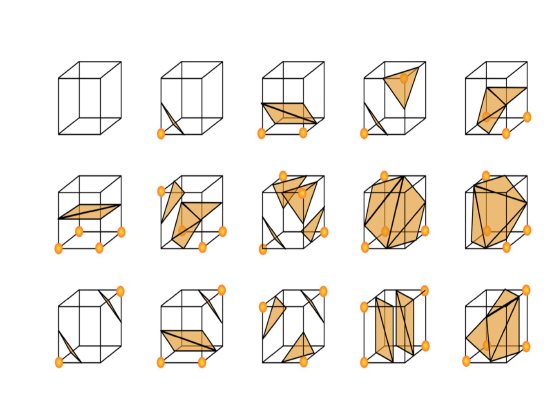
\includegraphics[width=0.4\textwidth]{shapes.png}
    \caption{Triangulated patterns} \cite[]{fang_zhao_wen_zhang_2018}.
    \label{fig:patterns}
\end{figure}

\enlargethispage{\baselineskip}

\section{SurfelWarp}
SurfelWarp is defined as "Efficient Non-Volumetric Single View Dynamic Reconstruction". It will present a standard graphics pipeline and GPGPU ("General-Purpose Graphics Processing Unit") computing can be utilised for efficient 
implementation of all data reconstruction operations \Citep*{SurfelWarp}. It eliminates the use of volumetric data structures, which represent resource-intensive volumetric operations such as dense deformation field updates, volumetric fusion, and marching cubes.
This represents a significant performance improvement as the explicit surfel representation allow to directly recover from tracking failures or topology changes as proposed by \citeauthor*{SurfelWarp}.

\subsection{Overview}
As illustrated in figure \ref{fig:surfelmetho}, SurfelWarp is built in a frame by frame methodology to process an input depth stream data source. 
When a new depth image is received, the deformation field that is aligned to the reference frame geometry will be solved. 
This is calculated by starting the deformation field from the previous image, which is followed by an iterative optimization problem similar to \Citet*{newcombe_fox_seitz_2015}.
Once the deformation field is updated, the data fusion process is carried out. This will trigger an accumulative process to fuse the current depth observations into a geometrical representation. 

The deformation field $ W = \{[p_j \in R^{3},\sigma_{j} \in R^{+} ,T_j \in SE(3)]\}$ where $j$ is the node index, $p_j$ is the position of the $j^{th}$ node. $\sigma_j$ is the radius parameter, $T_j$ is the 6DoF transformation.
For any point in "x" the deformation can be interpolated by equation \ref{eq:deffield1}
\begin{equation}  
  W(x)=normalized(\Sigma_{k \in N(x)} w_{k}(x) \hat{q_k})
  \label{eq:deffield1}
\end{equation}

\newpage
\begin{figure}%this figure will be at the right
    \centering
    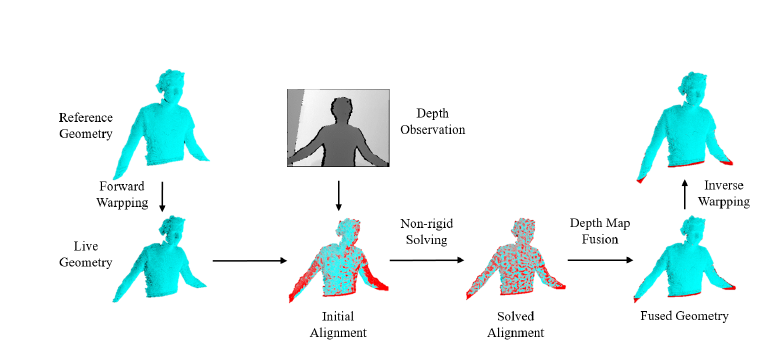
\includegraphics[width=0.95\textwidth]{surfelwarp1.png}
    \caption{SurfelWarp methodology }\cite[]{SurfelWarp}.
    \label{fig:surfelmetho}
\end{figure}

From equation \ref{eq:deffield1} the following components can be described:
\begin{itemize}
  \item $N(x)$: is the closest set of points x
  \item $W_{k}(x)$:  is the weight that can be computed as $\exp{(-\frac{\ | {x-p_k} \ |^{2}_2 }{2\sigma^{2}_k})}$
\end{itemize}

A surfel $S$ could be described as the composed tuple in which the following components can be modelled:
\begin{itemize}
  \item position : $v \in R^3$ 
  \item  normal  : $n \in R^3$
  \item  radius : $r \in R^+$
  \item confidence : $c \in R$
  \item initilization time : $t_{init} \in N$
  \item most recent time : $t_{observed} \in N$ 
\end{itemize}
Therefore, a surfel can be illustrated by the deformation of field $W$ in equation \ref{eq:deffield1} \citep{SurfelWarp}.
Furthermore, the deformed vertex position  and normal can be modelled with the following equations:
\begin{equation}
  v_{life}=W(v_{ref})v_{ref}
  \label{eq:deformed vertex}
\end{equation}
\begin{equation}
  n_{life}=rotation(W(v_{ref})n_{ref})
  \label{eq:deformed vertex normal}
\end{equation}

From equations \ref{eq:deformed vertex} and \ref{eq:deformed vertex normal} $v_{life}$ and $n_{life}$ are the deformed vertex position and normal.
Whereas $v_{ref}$ and $n_{ref}$ correspond to the vertex position and normal before the deformation process. 
\enlargethispage{\baselineskip}

\subsection{Depth Map Fusion \& Warp Fiel Update}
In order to get the warp field estimate, it is necessary to perform a mathematical prediction of the visibility of the live surfels models $S_{life}$ with the proposed method of \Citet*{newcombe_fox_seitz_2015}
to cast the deformation estimation into an optimization problem.
The estimation process is performed by predicting the visibility of life surfels $S_{life}$.
\begin{figure}[ht]%this figure will be at the right
  \centering
  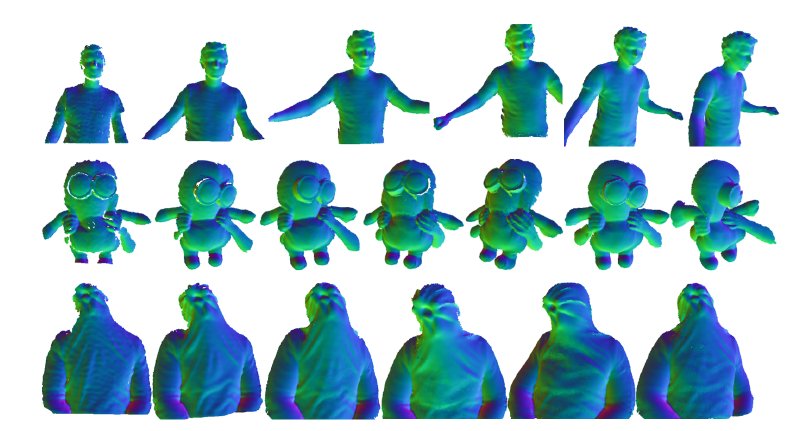
\includegraphics[width=0.9\textwidth]{surfelwarp2.png}
  \caption{SurfelWarp Reconstruction}\cite[]{SurfelWarp}.
  \label{fig:surfelprocess}
\end{figure}

Similarly, to the approach of \citet{keller} the life surfels $S_{life}$  are rendered as an overlaped disk shaped surface splat. These shapes are spanned by the position $V_{life}$ 
,normal $n_{life}$ and radius $r_{life}$ of the live surfel $s_{life}$.
With all these parameters it is possible to model the warp field based on the Dynamic Fusion framework proposed by \citet*{newcombe_fox_seitz_2015}.

Once the deformation is solved, the depth map fusion obtained from sensors along with the warp field update will perform data fusion in the live frame. 
This live frame warps the live surfel back to the starting reference frame. Afterwards, the warp field is recurrently updated based on the new observed surfels reference. This process can be exemplified with figure \ref{fig:surfelprocess}.

\chapter{Methodology}
As mentioned in the initial section, this project is focused on engineering design. Hence, it will be focused on creating a prototype for a 3D scanner. 
This includes the hardware and the software for the 3D model reconstruction, from which this section will be focused on the 3D model data reconstruction of the project.
The methodology will be divided into 3 sections that include: 


\begin{itemize}
  \item Data Acquisition
  \item Conceptual Design
  \item Design Implementation
\end{itemize}


\section{Data Acquisition}
As mentioned above the project can be described as an engineering design problem, whereby this approach includes the 3D software reconstruction model components for a 3D scanner. 
This includes gathering sensor data from the model that will be scanned. Many of the possible ways to gather data can be performed with commercially available sensors as proposed by \citet*{article}.

\citet{3D_scann_cultural} mentions that many 3D software reconstruction frameworks similar to Dynamic or SurfelWarp use commercially available sensors.
One of the most common approach to get data for 3D scanning will be to use RGB-D cameras. The proposed sensor that will be used for data acquisition is the 
\textbf{"Intel RealSense D435i"}. This Sensor is an depth camera with a stereo solutoin which is used in a wide variety of applications which include: 
\begin{itemize}
  \item Robotics
  \item 3D Scanning
  \item Skeleton and Human Tracking
  \item Drones
  \item Objects Measurement
  \item Facial Auth
\end{itemize}
\enlargethispage{\baselineskip}
Therefore, making this camera ideal for this project application.
\begin{figure}[h]
  \centering
  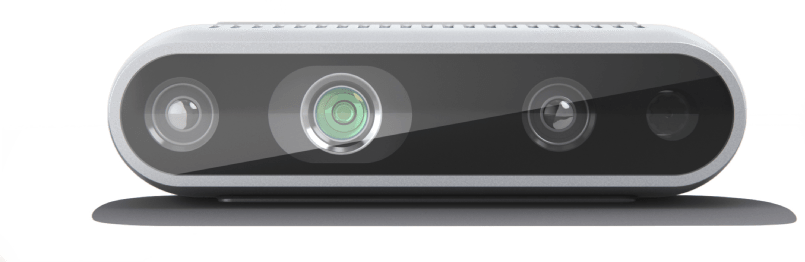
\includegraphics[width=0.9\textwidth]{d435i-1.png}
  \caption{Intel RealSense D435i}\citep*{intelrealsense}.
  \label{fig:d435i}
\end{figure}

This model of camera has a proprietary software development library and SDK which is used to interact with the computer. This SDK will allow calibrating the camera and 
obtain certain calibration parameters that will be used for data acquisition. 
Furthermore, there is a software wrapper that will allow connecting with ROS (Robot Operating System). This ROS wrapper will allow interacting between the middleware, which is ROS, the camera, and the computer. 
With aid of this wrapper, it is possible to integrate all the components of ROS and the camera. 
One of the benefits of using ROS is that it allows recording a certain set of data based on the information that is being acquired by the sensor. 
The wrapper will start the camera based on different configuration and it will publish data both RGB and depth images in the following topics:

\begin{itemize}
  \item  /camera/color/camera\_info
  \item  /camera/color/image\_raw
  \item /camera/depth/camera\_info
  \item /camera/depth/image\_rect\_raw
  \item /camera/extrinsics/depth\_to\_color
  \item /camera/extrinsics/depth\_to\_infra1
  \item /camera/extrinsics/depth\_to\_infra2
  \item /camera/infra1/camera\_info
  \item /camera/infra1/image\_rect\_raw
  \item /camera/infra2/camera\_info
  \item /camera/infra2/image\_rect\_raw
  \item /camera/gyro/imu\_info
  \item /camera/gyro/sample
  \item /camera/accel/imu\_info
  \item /camera/accel/sample
  \item /diagnostics
\end{itemize}
The above topics will contain all the data that the sensors perceive in real-time. As can be seen from the above list, there will be data for the RGB, Depth sensors, Infrared sensors, IMU as well as all the extrinsic and status of the camera parameters. 
Furthermore, all this data will be processed with different formats such as raw or compressed. Based on the data perceived from these topics, it will be possible to create 3D point clouds in realtime and run 3D data reconstruction frameworks such as Surfelwarp as the sensors acquire and perceive the environment. 

On the other side, ROS allows to record data from the above topics. From the above topics, it is possible to record the data messages as a "rosbag" or "bag", which is a file format in ROS for storing message data. Hence it will allow recording the data that the camera is sensing. 
Furthermore, these bags allow subscribing to specific topics, which implied that only the required topics will be stored for 3D data reconstruction and storing the data of the received message in an efficient file structure. 
The data acquisition process for the development phase will be performed by storing several rosbags, to be used in the development phase of the 3D reconstruction for the scanner.

\section{Conceptual Design}
The conceptual design will be focused on the development of the 3D software reconstruction for a 3D scanner. 
The Initial design will be to test with the field of view of the Intel RealSense D435i for both RGB image and Depth image sensors. From which for the Field of view (H × V × D) of the RGB corresponds to 69.4° × 42.5° × 77° (±3°),
whereas the depth of the field of view for the Depth sensor corresponds to 86° × 57° (±3°)\citep*{intelrealsense}.

Based on these results there will be a testing and evaluation phase, which involves evaluating what is the ideal configuration for the Camera. The ideal configuration will be based on which pose the sensor will be able to obtain the most accurate and useful data. 
Hence a mannequin will be used for this testing purpose from which the ideal pose for the sensor will be determined. 
%\enlargethispage{\baselineskip}

Once the ideal pose for the sensor is found, there will be the need to evaluate and test which is the fastest and most accurate way to obtain data of the model. All the testing purpose will be performed by recording several rosbags and visualise them.
This has the intent to find the ideal location and number of all sensors that will be able to scan all the model. With this method, it will be possible to determine the speed and reliability of the Scanning process. 
Based results of this it will be possible to determine a prototype for the mechatronic design of the scanner as well as the methodology of how to fuse the data and run the 3D reconstruction framework. 

The Design implementation of the 3D reconstruction software will be to adapt and adjust the 3D modelling data reconstruction frameworks. Hence, it includes developing the corresponding ROS nodes that will allow to use the data from multiple sensors and fuse it. 
With the fuse data, the intent is to run the 3D reconstruction framework which will output the Scanned model. 

Once the process of generating the 3D scanned model is stable. The software will be ported to a small machine such as the Intel NUC, which is a small form factor computer. 
The software will be installed into the Intel NUC with the purpose to be incorporated with the mechatronic design of the 3D scanner. This will facilitate easy operation of the entire 3D scanning device.
\begin{figure}[ht]
  \centering
  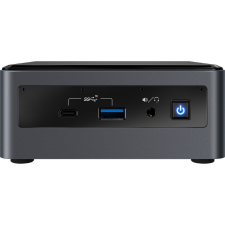
\includegraphics[width=0.4\textwidth]{Nuc.png}
  \caption{Intel NUC}\citep*{IntelNuc}.
  \label{fig:NUC}
\end{figure}


\chapter{Project Management}
This section will provide guidelines and illustrate the management procedures that will be implemented into the feasibility and development of the software reconstruction for a 3D Scanner. 
It provides a projected timeline for deliveries and identifies specific methodologies implemented for the execution of the project from the beginning to the competition of all tasks.
The project plan will be updated throughout the development of the project to reflect deliverables that may be affected by potential shortfalls.
In order to prevent this, it will be necessary to circumvent any affected task and resolve it in an adequate timely manner. 
This will be a collaborative project, that involves creating the hardware device that will allow placing the sensors, the 3D data reconstruction of the Model, and the post utilization of the model for different uses such as testing virtual clothes. 
As the agreed allocated task was the 3D data reconstruction this section and document will be focused on the 3D software for data reconstruction.

\section{Scope}
There are multiple ways in which a 3D scanner is defined. Many connotations include creating the actual hardware of the device or how is the software going to be developed to create a 3D model. 
Based on this, the scope of this project component is to develop and deploy the software for 3D reconstruction of a scanning device as it was previously mentioned. 
The software will retrieve data from multiple sensors and cameras to then perform data fusion and create a 3D representation of the model that is scanned. Whereas the other components of the collaborative task will include the device creation as well as different applications for the obtained models. 

The allocated 3D reconstruction part will include two phases to approach the engineering design problem that is targeted. 
The initial phase will be focused on gathering data from a wide variety of sensors that include RGB and Depth Cameras and test which is the most effective way to collect data of the model. 
The second phase will be to develop a framework and methodology to fuse the acquired data from the sensors to create a 3D model representation of an object, which in this particular case will be a person. 
The project will span for over 35 weeks inclusive of Spring 2020, Summer Break 2021, and Autumn Session 2020 UTS academic semesters. This will include working with various teams that oversee the development of the hardware prototype as well as the uses of the model. The subsequent details are located in the sections below. 

\subsection{Project Specifications}
It is important to outline all the specifications of the project in order to ensure, that the design will satisfy the purpose and it matches the scope of the project. As this is a collaborative project, the other team member will need to elaborate their corresponding details for their allocated sections. 
All of this will be reflected on the Work Breakdown Structure and Gantt Chart, however, the details for the 3D data model reconstruction will be explained below.  

\subsubsection{Sensing \& Data Acquisition}
There are multiple ways to achieve data acquisition that will satisfy the project. The proposed way would be to use sensors, especially, RGB and Depth Image Cameras
The sensors should be able to provide with the following:
\begin{itemize}
  \item RGB  Colour images of the object or model
  \item Provide Depth images  to get Distance for every point in the image
  \item Have a large enough field of view that could fit the entire object or model
\end{itemize}
The data acquired from these sensors should be reliable to ensure the fidelity of the final 3D reconstructed model. These data sensors will be converted to Point clouds via data fusion, where each point in the model will be mapped. Hence creating a 3D reconstruction model where its corresponding location in space is known. 
Therefore, the proposed sensor that will be used will be the Intel RealSense D435i. From which the SDK and ROS wrapper will allow to obtain the data and facilitate the process. 

\subsubsection{Data Fusion \& Timing}
Once the data is acquired from the sensors it will be required to fuse the data to be able to create the model.
 Data fusion is proposed to be performed in Realtime as the objects are scanned. This data fusion process will be performed by processing the data from multiple sensors and running them to a 3D reconstruction framework such as SurfelWarp. 
Thus, creating a visualization preview of the object or person scanned. 

On the other hand, the timing would be critical, as in most application the scanning time should not take more than a couple of minutes that could vary from 2 to 5 minutes.
Therefore, ideally, the 3D reconstructed model from the scan should finalize within that time frame.

\subsection{Project Overview \& Deliverables}
The project overview can be exemplified in figure \ref{fig:ConstrainedWBS} and it is associated with all the possible deliverables for the project
\begin{figure}[ht]
  \centering
  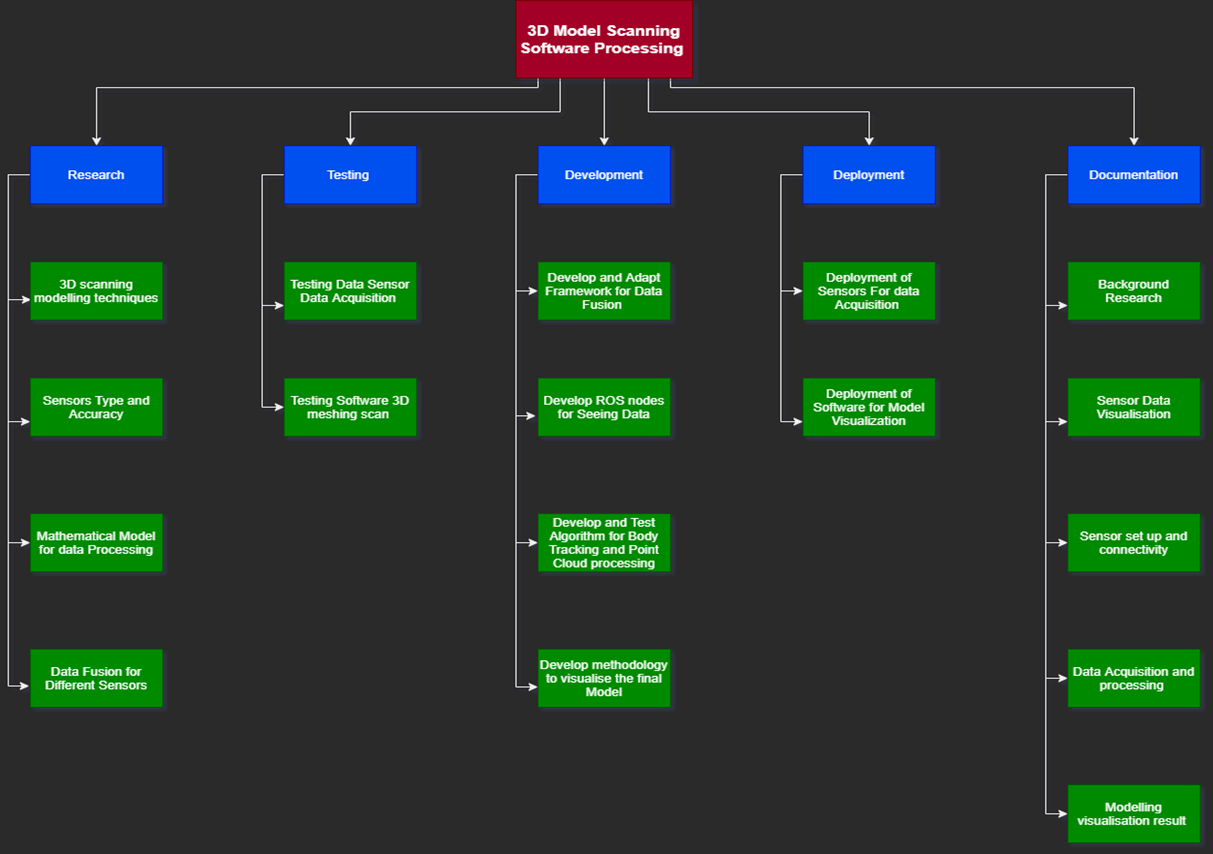
\includegraphics[width=0.9\textwidth]{ConstrainedWBS.png}
  \caption{Constrained WBS for 3D data reconstruction component}
  \label{fig:ConstrainedWBS}
\end{figure}

Furthermore, it is imperative to demonstrate and illustrate the entire work break down the structure of the project. This will include other sections and components such as: 
\begin{itemize}
  \item Developing the hardware device to do the scanning methodology. 
  \item Integrating the sensors for data acquisition and 3D reconstruction for the model.
  \item Uses the model for different applications. 
\end{itemize}

The details will be located in the appendix on figure \ref{appendix:wbx}
 
\section{Project Timeline}
\begin{wrapfigure}{r}{0.5\textwidth} %this figure will be at the right
  \centering
  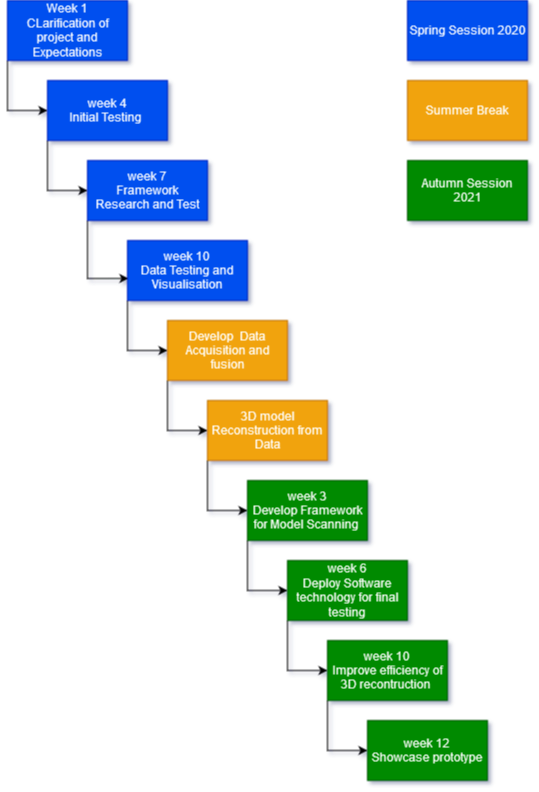
\includegraphics[width=0.5\textwidth]{timeline.png}
  \caption{Transformation Between Depth Video to Warped canonical Model}
  \label{Fig::timeline}
\end{wrapfigure}

The timeline shown in figure \ref{Fig::timeline} depicts the problem-solving approach that is proposed in order to fully complete the optimum deliverable for the project. 
The below image summarises and synthesis the process in a waterfall approach. As there must be a certain number of deliverables that needs to be accounted for an agile approach would not satisfy the needs of the individual components. 
Once most components are developed with the waterfall approach, an agile methodology will be necessary to integrate all the other components of the project.

These include:
\begin{itemize}
  \item Hardware development of device
  \item 3D software for data reconstruction and modelling 
  \item Uses and applications of 3D model
\end{itemize}

The proposed timeline from start to finish for the proposed project will be approximately  35 weeks. Including both UTS academic semester (Spring 2020 \& Autumn 2021) and the corresponding university summer break holiday.
All the detailed tasks and proposed deadlines are located in the Gantt Chart, located in the appendix.
The proposed plan is inclusive of contingency scenarios as extra allocated days are added for different tasks. Any potential date changes will be updated accordingly in the plan,  to keep the project completion as accurate as possible for the 3D reconstruction component.  

\newpage
\section{Progress \& Milestones}
Any project must identify and define particular milestones for the project. 
Once the milestones are identified, they can be properly analysed to establish the corresponding requirements, processing, development and execution. 
After all these parameters have been established a corresponding timeline could be proposed. All these milestones will be considered for the 3D model reconstruction component. 

This project component includes two particular and independent phases. 
Phase one will include the design proposal and data acquisition and processing, whereas phase two will focus on data fusion and 3D model data reconstruction.  
These phases could be subdivided five into smaller interdependent subprocesses that would contribute to the corresponding milestones that are part of the project deliverables. 
Thus, a holistic approach should be implemented with a waterfall implementation. The six major work areas include:

\begin{itemize}
  \item Research and Conceptualization
  \item Testing 
  \item Evaluation
  \item Development
  \item Deployment 
  \item Documentation
\end{itemize}

The section below will delve into deeper detail of each project and illustrate the major milestones within itself. All do this will be illustrated for the 3D data model reconstruction component. 
All the other details for the other components are located in the work breakdown structure located in the appendix in figure \ref{appendix:wbx}. 

\subsection{Milestones and Stages}
\subsubsection{ Stage 1: Research and Conceptualization }
The research component of this project will rely on exploring different robotics parameters and 3D data modelling reconstruction. 
The corresponding limitations will be analysed via research into different 3D reconstruction techniques that have been developed and what are the current developments in this 3D scanning field. 
The already existing solutions will aid to conceptualise the project to ensure optimal functionality that will produce an accurate 3D scanned model of persons or objects
Potential solutions for software implementation will be investigated in detail to grasp the basics of the different algorithm and how they behave in different scenarios. 

Furthermore, different kind of sensors will be investigated to use the most appropriate equipment to grasp the data. Different data fusion frameworks will be analysed to make a collection of them in order to develop the data reconstruction prototype. 

A recommendation will be made to the supervisor and team regarding optimal sensors that could be implemented and what type of data reconstruction could be utilised. 
\enlargethispage{\baselineskip}

\subsubsection{Stage 2: Testing}
The testing phase for the 3D reconstruction component will be based on testing the different features and component that the d435i has available. The corresponding included SDK’s will be used to see the camera parameters and different ways to grasp the Data. 
Furthermore, different tools will be tested to mesh raw data to test the reliability of the acquired data. 
On the other side, the meshing components will allow grasping the idea of how different techniques allow doing model meshing under different circumstances for the 3D data reconstruction framework. 

All the parameters from the testing phase that include the test of single and multiple sensors for data acquisition. Similarly, an experimental test for sensors synchronization and calibration will be perform accordinly in the testing phase. 
Based on these parameters the evaluation of all the components will be perform accordingly before the development and deployment stages.

Moreover, there is the need to test how the different 3D reconstruct frameworks perform under different scenarions and conditions and evaluate the performance in order to start the development process.

\subsubsection{Stage 3: Evaluation}

The evaluation stage will be performed under the testing phase. From the obtained results there will be a corresponding team evaluation in which it will be assessed the use of single or multiple sensors. 
From this, it will be possible to obtain a clear insight into how many sensors will be necessary for the implementation. All these processes will be evaluated based on how the data is received and how it will be integrated with the final mechatronic prototype of the 3D scanner. 
This will be evaluated based on the requirements on how much data is necessary for the entire model as well as how much data can each sensor obtain based on the field of view.

Similarly, there will be a corresponding evaluation process on how to enable multiple sensors synchronization. This will be tested and evaluated to ensure that the sensors will work simultaneously and that these will be able to acquire data synchronously. 
On the other side, it is crucial to test the accuracy of the sensors. Therefore it is a must to enable multiple sensor calibration. For this process, it will be necessary to obtain the camera calibration parameters. This includes obtaining the intrinsic and extrinsic parameters. 
Based on this it will be possible to obtain the distortion of the camera and it will be possible to calibrate each sensor accordingly.
With these results, it will be possible to evaluate how multiple sensors  will interact with each other and how the calibration process will be performed for the development and deployment stages

On the other side. it is crucial to assess the performance of Dynamic Fusion and SurfelWarp. 
These will include evaluating the performance under different scenarios and with different models. Also, the speed, accuracy and results will be assessed. 
Based on the results, it will be possible to choose the appropriate framework and to plan potential modifications that might need to be developed in the development stage.


\subsubsection{Stage 4: Development}

The development phase will consist of developing and adopting a framework for Data fusion. The data will be provided with the sensor that was chosen from the previous stage. 
The results obtained will allow to fuse all the data from all the components from the different sensors and visualise them into a single output.

Furthermore, there will be the development of the ROS nodes that will allow collecting the data in real-time that will be pass onto the data fusion framework.
The ROS nodes will allow to properly map all the sensors and allow them to work simultaneously. Additionally, there will be the development and corresponding test for Body tracking of the scanned models and to convert the data from the sensors into Point clouds. 
These point clouds will be tested for accuracy of the Scanned data in the visualised model. 

From this acquired and processed point clouds a methodology will be developed to work in conjunction with the Data fusion framework to visualise the final model. 
All these processes will be tested under different conditions to ensure that it will work under most circumstances and will allow a much easier deployment process. 

\subsubsection{Stage 5: Deployment}
The deployment phase will be subdivided into two main tasks. The initial one  consists of the deployment of all the sensors that will be utilised for data acquisition. 
This will include in deploying and installing the sensors into the actual hardware device that will be used. 
These Sensors will be mounted and interconnected between then for enhanced sensing. This will be worked in conjunction with the hardware team. 

Similarly there will be the deployment of the software tools that include the ROS nodes, Data fusion Framework and Model visualization methodology. 
All of this components will be deployed into the final device that is part of the hardware team. 


\subsubsection{Documentation}
The documentation process is one of the crucial components of this project. 
Especially for the 3D data reconstruction component. All the corresponding stages of the research, testing, development, and deployment will have their proper documentation with a high level of detail. 
There will be the corresponding documentation regarding the background research of the project. 
It will include all the necessary research, use to determining the scope of the project and what are the current solutions for it. 

Similarly, the documentation for all the sensor data visualization will include what type of sensor was used. It is characteristics, and what SDKs and libraries were used. 
The corresponding method of visualising the data will be documented as well as all the commands necessary for its use. 
Furthermore, all the necessary diagrams for connections and set up will be fully documented. As this will help massively the other teams. 

There will be a detailed explanation of how the data acquisition process is carried out and what are the methodologies are used for data fusion. 
This also includes topics such as: what are the best scenarios and circumstances for using the developed technology. 
Finally, there will be the included detailed explanation of how the 3D model is generated. 
All other content such as risks a limitation will be included as the project is developed.

\subsection{Gantt Chart}
Please refer to Appendix, figure \ref{appendix::gant}, to visualise the Gantt Chart. The proposed Gantt Chart provides a detailed timeline, that includes dates and duration for each milestone. 
It will include milestones that are part of the hardware team and the use case team. Therefore, it will include all the proposed milestones for the entire project. 
It is important to know that the proposed timeline and dates might change, especially the ones that belong to the other teams (hardware and use case). 

It is crucial to note the following:
\begin{itemize}
  \item The work schedule and load differ between each academic semester. Thus, extra time was added to counteract this effect.
  \item The finalisation date and showcase were planned for the last week of the Autumn 2021 semester. 
  \item There is a continuation of work through the UTS summer break with the purpose of maximising efficiency. This is reflected on the Gant Chart.
\end{itemize}

\section{Resources}
Resource planning is essential for any successful project. 
Different steps and different teams will require different resources and support. For this project, the principal resources can be split into human and technical. 

\subsection{Human Resources}
As this project is non-confidential, it will not have any external relations. Hence, the main people involved in every component are the following:
\begin{description}[style=nextline]
  \item[Academic Supervisor – Dr Teresa Vidal Calleja] Teresa is the Deputy Head of School (Research), School of Mechanical and Mechatronic Engineering as well as Core Member for CAS - Centre for Autonomous Systems. Her Interest Include Robotic perception, automatic recognition, alternative sensing, visual SLAM, aerial and ground robot’s cooperation, and autonomous navigation and manipulation.
  \item[Hardware Component lead – Asher Katz] Asher is the other capstone student of this project. He will oversee developing the hardware ad mechanism for the scanning device.
  \item[Use cases Component Lead – Mark Liu] Mark will oversee the use case of the project. He will use the 3D scanned models to try out clothing sizes virtually for different fashion items.
  \item[Cedric Le Gentil] Cedric will help in the process of creating the 3D scanner as well as facilitating the use case to adapt fashion items to the scanned models.
  \item[Nico Pietroni] Nico will be in charge of making the adaptation process between the 3D scanned models to the use case. Where he will develop the software for adding the clothes meshes to the 3D scanned model.
\end{description}

\subsection{Technical Components }
The technical components will include all the required sensors and software that will be implemented. The following resources are critical for the development, testing and deployment phases of the project. 

\subsubsection{Sensors}
The proposed sensor that will be used for both testing and development is the Intel RealSense D435i. These components will need to be purchased to start with the project. Is estimated that the price for the D435i is 200 \$ USD
These sensors are crucial and will need to be imported from the US. 

The corresponding software controllers and SDK for these sensors are available online and would only need to be installed and compiled. 
Depending on the outcome of the testing phase it will be necessary to determine the number of sensors that would be used. Hence the total overall price for the sensor is not fully established yet. 

\subsubsection{ROS}
As mentioned previously ROS (Robotic Operating System) is a robotics middleware. It provides with the necessary services that are designed for a computer cluster that includes : 
\begin{itemize}
  \item Hardware abstraction
  \item Low-Level device control
  \item Synchronization for multiple sensors
  \item Real-time data acquisition of recording for sensors
  \item Sensor Data visualization in real-time.
\end{itemize}

ROS is free and can be installed easily in a Linux machine. All the proposed sensors have the corresponding ROS driver that will allow connecting the sensors with ROS with ease. 
This middleware will allow to collect, synchronise, and initialise all the sensors. As well as visualise all the acquired data in real-time. ROS allows an easy implementation of the framework for data fusion and Model reconstruction. 

\section{Uncertainties \& Risk Control}
All projects face some particular level of unforeseen risks and uncertainties. Good project planning will consider all possible areas of failure and introduce mitigation plans to try to control and prevent the consequences.  
All these uncertainties and risk matrix will be considered only for the 3D model data reconstruction component. The other components will need to be considered by the responsible respective teams. 

\newpage
The Uncertainties of the project float around the next parameters:
\begin{itemize}
  \item How is the 3D data reconstruction going to work.
  \item How accurate is the data acquisition from the sensors.
  \item How long is the scanning process going to take. 
  \item How long is the Testing and developing processes going to take. 
  \item How is the deployment process going to work.
  \item How is the use case going to be applied for virtual clothing.
\end{itemize}

On the other side, the risk Matrix will explore all possible identified risks of the project. 
There is a severity scale from low to high that will illustrate the potential impact on the project and whether it will hinder the competition of itself.
 Additionally, the likelihood of each risk is analysed to reflect the priority risk mitigation. 
The risk mitigation table will be located in the appendix on table \ref{appendix:risk}. 

\section{Communication Management}
The predicted communication plan was completed and developed after identifying all key stake holders, participants, communication channels for this endeavour. The major stake holders include:
\begin{itemize}
  \item Capstone supervisor
  \item Hardware device capstone student
  \item User case team
  \item Engineering research preparation staff
\end{itemize}
As mentioned before the planned proposed time is expected to cover 35 weeks (27/7/2020 -30/6/2021). This includes both UTS academic semester as well as UTS summer break. 
The proposed communication plan will be located in the appendix on table \ref{appendix:ComunicationPlan}. 

\chapter{Progress Statement}
The progress of this project is running accordingly to the plan of the Gantt Chart as reflected in figure \ref{appendix::gant}.
This section will discuss in detail the findings of all the work that has been done to date.
This includes researching the type of sensors that could be implemented such as the Intel RealSense D435i. 
Furthermore, there was a research stage that included to browse several 3D reconstruction frameworks and how these perform. 
On the other side, it was also necessary to research the components of the underlying frameworks and how it is constructed. Based on this, it was a must to investigate the dependencies 
are necessary to install these frameworks into the computer in order to start the 3D software reconstruction. 
Furthermore, all the project planning was developed. This includes creating the communication plan, risk matrix as well as the Gantt Chart and all the methodology that will be implemented on the project. 

On the other side, several tests were performed with the purpose of gathering data of the model. These tests were performed with the purpose to test the different methods in which it was possible to gather data for a model.
For these tests, a mannequin was used as the test model. Please refer to figure \ref{fig:mane}.

\begin{figure}[ht]
  \centering
  \includegraphics[width=0.5\textwidth]{manequin.jpg}
  \caption{Manequin used for testing}
  \label{fig:mane}
\end{figure}


From these tests, it was possible to obtain RGB and Depth images, that will allow seeing the Field of view of the sensor. Furthermore, it allowed to see and plan, the potential mechatronic design of the scanner and the number of sensors that could be used in the final design.
The result of this test was that it was necessary to use a certain number of sensors in different positions in order to obtain as much information and data as possible for the scanned model. 

In contrast, another test was performed with the purpose of gathering data from different positions. Hence, scanning a mannequin from different angles with the purpose of gathering the most data as possible. 
From these tests, it was possible to obtain the best configuration position for the camera, with the purpose of maximising the Field of View of the RGB and Depth Sensors.
Furthermore, it allowed obtaining the 3D point clouds of the model in realtime, which allowed to have a preview of the scanned model.  

Based on these tests it was also possible to determine the requires distance that the camera has to be from the model in order to obtain a preliminary radius of the scanner mechatronic design.
This was done by observing the point clouds and via analysing the Sensor data in realtime. The RGB and Depth images acquire from these sensors can be observed on figures \ref{fig:scanRGB} and \ref{fig:scanDepth} respectively.
\begin{figure}[ht]
  \centering
  \subfloat[RGB sensor data results] {\label{fig:scanRGB}{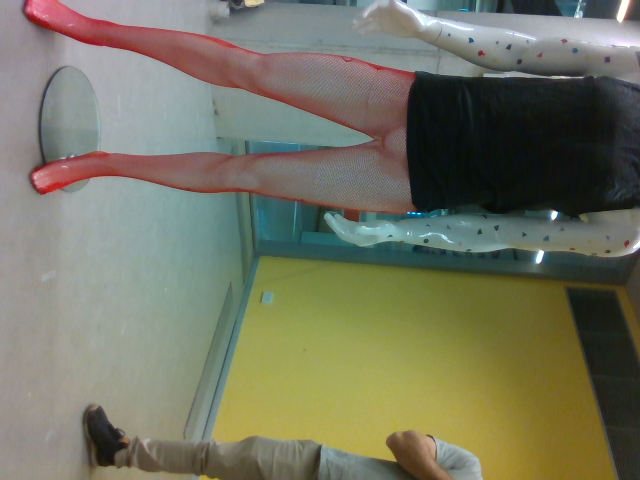
\includegraphics[width=0.6\textwidth, angle=90]{scan1.png}}}\hfill
 \subfloat[Depth image sensor data results]{ \label{fig:scanDepth}{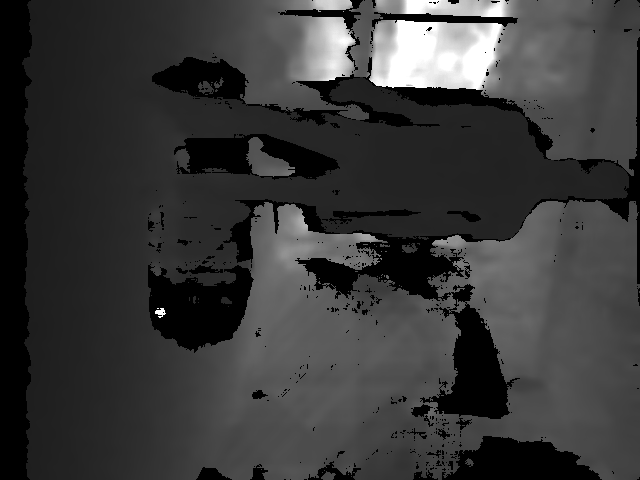
\includegraphics[width=0.6\textwidth, angle=90]{scan2.png}}}
 \label{fig::RGBD d435i}
 \caption{RGB \& Depth Image Data}
\end{figure}


\nocite{*}   % all not cited bib entrys are shown in bibliography ...
\bibliography{resources}


\appendix
\chapter{\vspace{-5.5cm}Appendix}

\begin{table}[!htb]
  \centering
  \makebox[\textwidth]
  {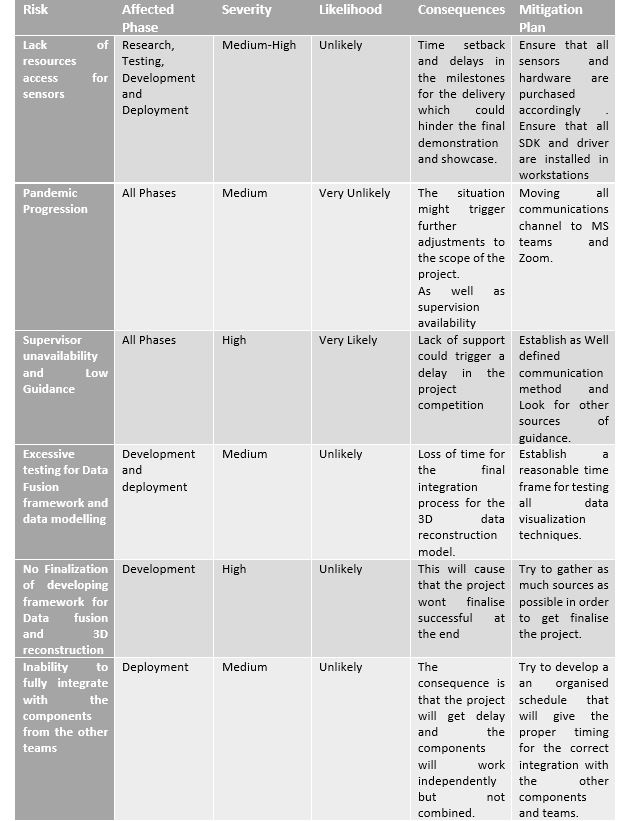
\includegraphics[width=1\linewidth]{Risk_matrix.png}    
  }
  \caption{Risk Matrix}
  \label{appendix:risk}
\end{table}

\newpage
\begin{table}
  \centering
  \makebox[\textwidth]
  {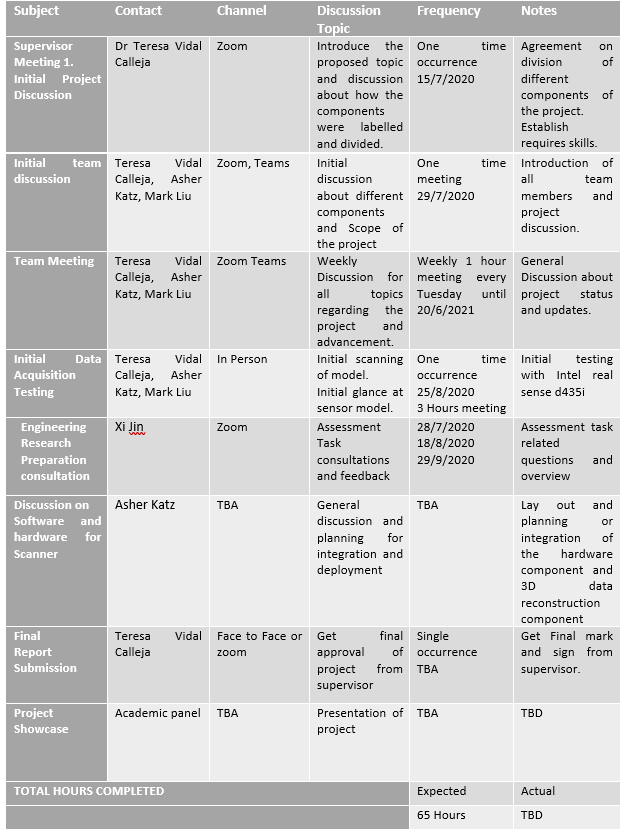
\includegraphics[width=1\linewidth]{ComunicationPlan.png}    
  }
  \caption{Comunication Plan}
  \label{appendix:ComunicationPlan}
  \end{table}    

\newpage 
\begin{landscape}
  \thispagestyle{empty}
  \begin{figure}
    \centering
    \makebox[\textwidth]
   
    \caption{WorkBreakDown Structure}
    \label{appendix:wbx}
    \end{figure}   
\end{landscape}

\newpage
\newgeometry{top=10mm, bottom=10mm,left=1mm,right = 5mm}  
\begin{landscape}
  \thispagestyle{empty}
  \begin{figure}
    \centering
    \makebox[\textwidth]
   
    \caption{Gantt Chart}
    \label{appendix::gant}
    \end{figure}   
\end{landscape}
\restoregeometry

\end{document}
